\chapter{Winston-Lutz test module} \label{chr:wlTest}

This chapter describes the structure, functionality and algorithms used in the W-L test module. For technical description and implementation in application see \autoref{sec:techWL}.

\section{Pylinac and coordinate space}

The module uses the Pylinac library (Winston-Lutz module) as its underlying framework. \cite{pylinac_wl_algorithm}. The coordinate system used in Pylinac conforms to IEC 61217 coordinate space. \cite{iec_61217}

\begin{figure}[H]
    \centering
    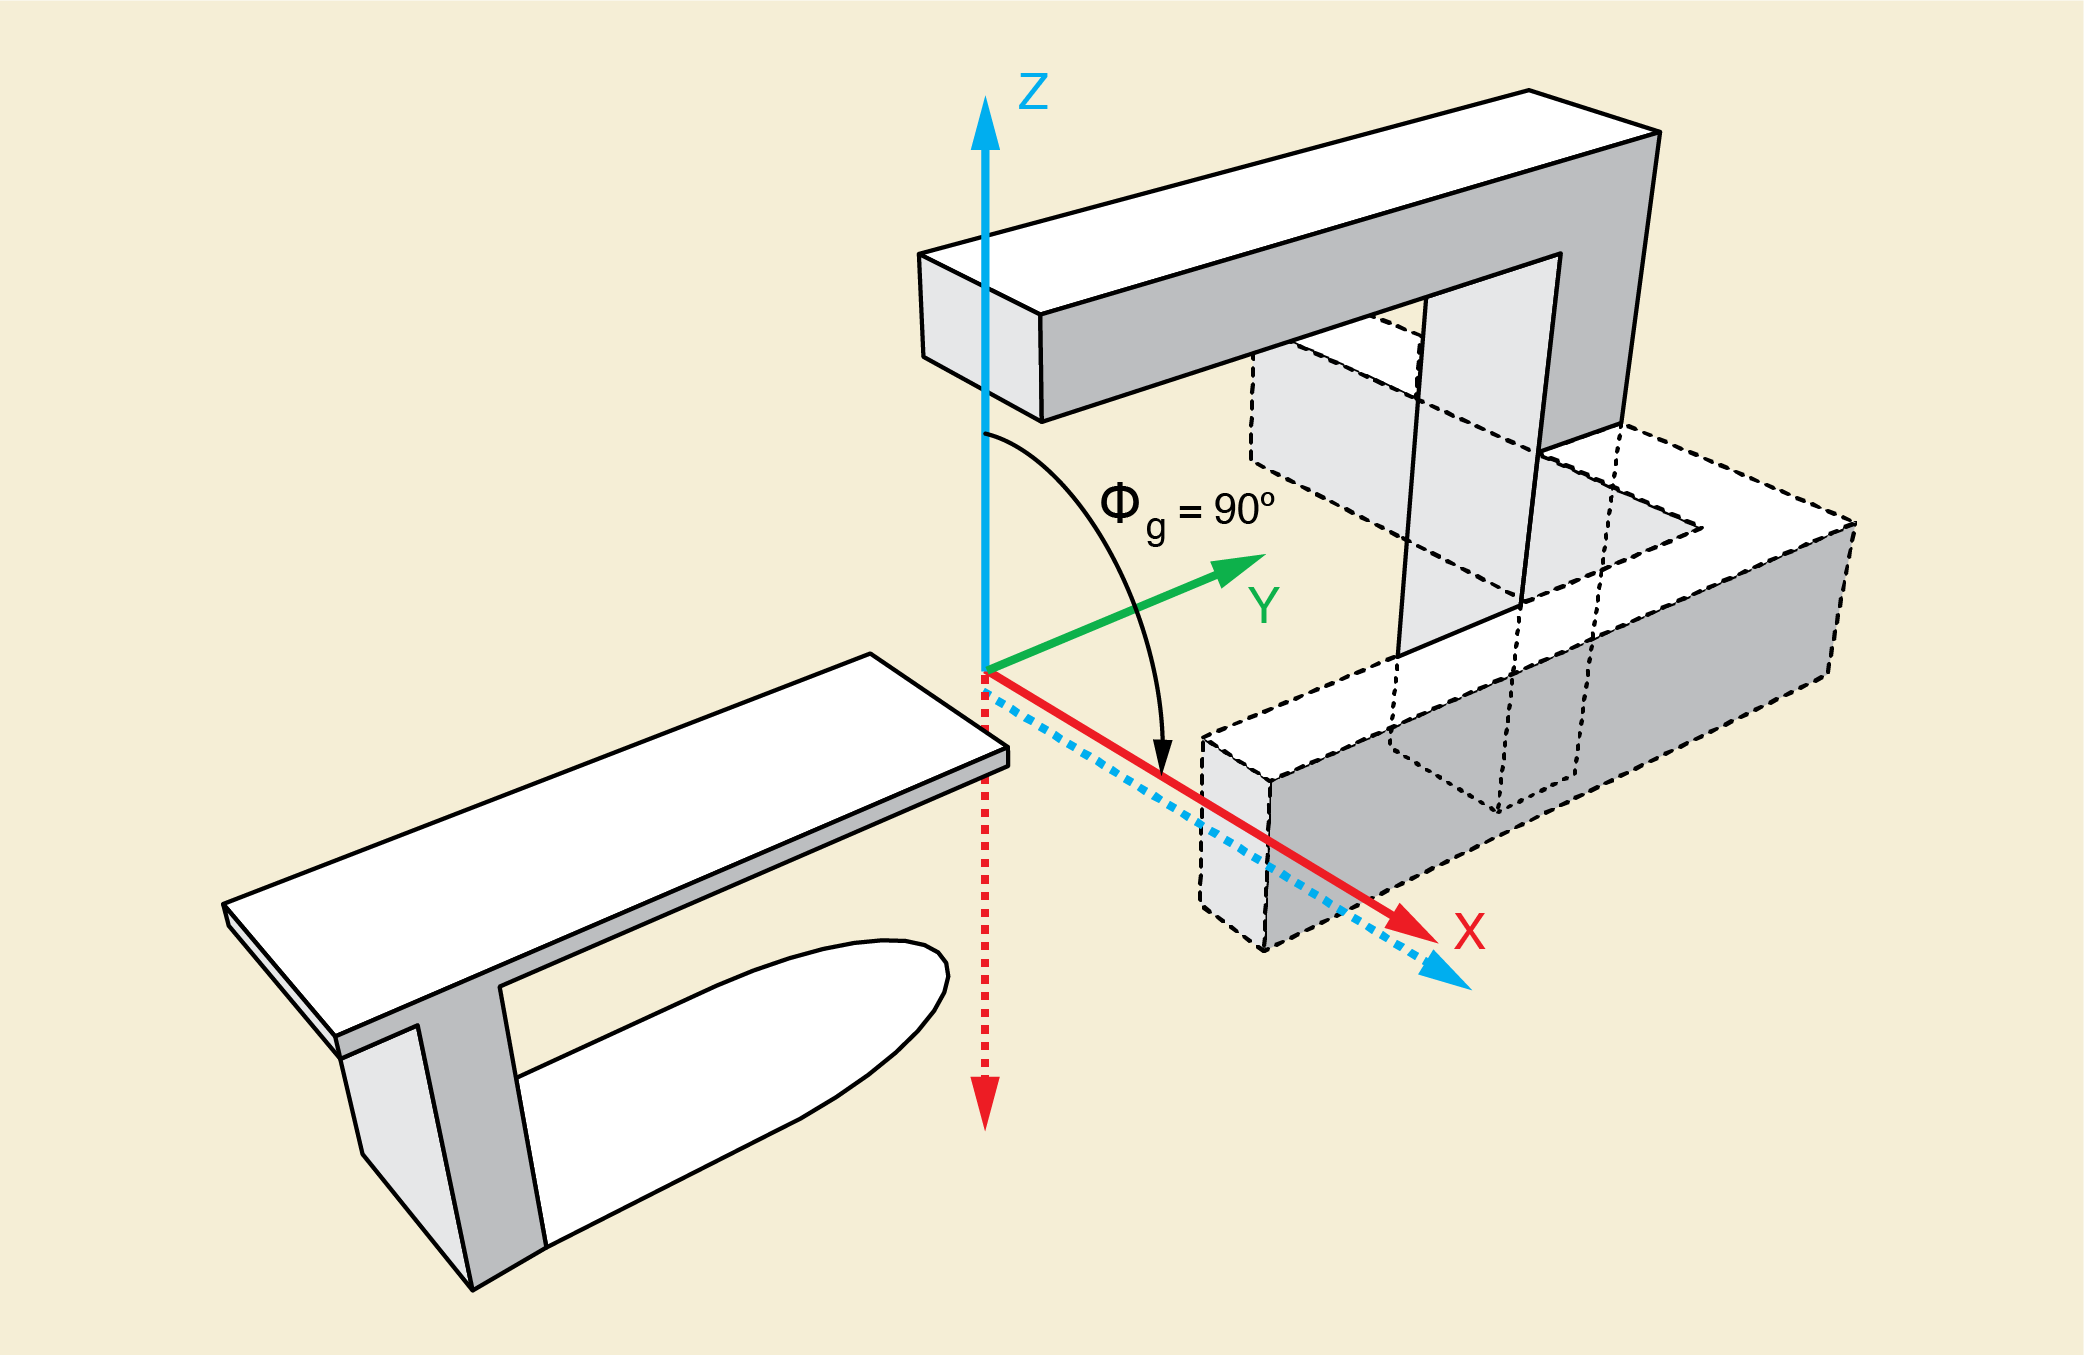
\includegraphics[width=0.7\textwidth]{Content/Images/pylinac_coordinate_space.png}
    \caption{Coordinate space used in Winston-Lutz pylinac module} \cite{iec_61217}
\end{figure}

The structure and algorithms described below are encapsulated in the Pylinac library, which provides an API to perform the test that uses them. The module described in the thesis performs the W-L test, using Pylinac's methods. However, the library returns raw data and plots, which are then processed and organised in the application to be presented concisely in the application frontend.

\section{Features}

\begin{itemize}

    \item \textbf{Couch shift instructions}

    Module provides feedback how to shift the couch to relocate the mechanical isocenter to match the radiation isocenter.

    \item \textbf{Automatic field and BB positioning}

    CAX and BB are found automatically, along with the vector and scalar distance between them.

    \item \textbf{Isocenter size determination}

    The 3D gantry isocenter size and position can be determined using back projections of the EPID images, independently of the BB position.

    \item \textbf{Axis deviation plots}

    Variations of the gantry, collimator, couch, and EPID are plotted together with their root mean square variation.

    \item \textbf{Isocenter visualization}

    The 3D plot of the isocenter and BB is generated.

    \item \textbf{PDF report generation}

    PDF report with all the above data summed up can be generated.
    
\end{itemize}

\section{Interface structure}

The module loads and processes EPID images and outputs resulting data in the form of numerical values, plots and images.

\subsection{Inputs}

\begin{itemize}

    \item Valid W-L test EPID images (defined in \autoref{subsec:wlPylinacAlgorithmRestriction})
    \item Size of BB
    
\end{itemize}

\subsection{Ouptuts}

\subsubsection{Numerical values} \label{sec:wlTestNumericalOutput}

\begin{multicols}{2}
\begin{itemize}

    \item Couch shift instructions
    \item Number of total images
    \item Number of gantry images
    \item Number of couch images
    \item Number of collimator images
    \item Maximum 2D CAX to BB distance
    \item Median 2D CAX to BB distance
    \item Mean 2D CAX to BB distance
    \item Maximum 2D CAX to EPID distance
    \item Median 2D CAX to EPID distance
    \item Mean 2D CAX to EPID distance
    \item Gantry 3D isocenter diameter
    \item Maximum Gantry RMS deviation
    \item Maximum Collimator RMS deviation
    \item Maximum Couch RMS deviation
    \item Maximum EPID RMS deviation
    \item Gantry + Collimator 3D isocenter diameter
    \item Collimator 2D isocenter diameter
    \item Couch 2D isocenter diameter
    
\end{itemize}
\end{multicols}

\pagebreak

\subsubsection{Plots}

\begin{multicols}{2}
\begin{itemize}

    \item In-plane Gantery displacement
    \item In-plane Epid displacement
    \item In-plane Collimator displacement
    \item In-plane Couch displacement
    \item Isocenter Visualisation
    
\end{itemize}
\end{multicols}

\subsubsection{Images}

\begin{multicols}{2}
\begin{itemize}

    \item Gantry wobble
    \item Collimator wobble
    \item Couch wobble
    \item Gantry images
    \item Collimator images
    \item Couch images
    \item GB Combo images
    \item GBP Combo images
    
\end{itemize}
\end{multicols}

\section{Algorithm} 

The algorithms presented in this section are not the author's work; they are adapted from the pylinac documentation \cite{pylinac_wl_algorithm}. However, these materials facilitate comprehension of the test methodology, the generation of results, and, consequently, the functioning of the application. For this reason, they are presented here.

\subsection{Algorithm allowances}

\begin{itemize}
    \item Images from any EPID can be used, with any SID.
    \item Even though BB distance from real isocenter affects 2D image analysis, it does not need to be near it to determine isocenter sizes.
\end{itemize}

\subsection{Algorithm restrictions} \label{subsec:wlPylinacAlgorithmRestriction}

\begin{itemize}
    \item The BB must be within 2.0cm of the real isocenter.
    \item The images must be obtained with the EPID.
    \item The BB must be completely within the field of view.
    \item The linac coordinate system must be IEC 61217.
\end{itemize}

\subsection{Algorithm definition}

\begin{enumerate}

    \item Find the field CAX

    Pixel span ($max - min$) is divided by $2$. Any pixels above the threshold are considered open field. Pixels are binarized and CAX is assumed to be in the centre of mass of the pixels.
    
    \item Find the BB

    The algorithm is described in \autoref{subsec:finding_BB}.
    
    \item Calculate couch shift vector

    Calculations as defined in \autoref{subsec:couch_shift}

    \item Backproject the CAX for gantry images

    Based on the gantry angle and $\xi$ (\autoref{eq:cax_bb_shift_matrix}), a 3D line projection of the CAX is designated. The origin is considered at BB. For this step, only images with the coach at angle 0 are considered.

    \item Determine gantry isocenter size

    Using the above, the maximum distance to any line is minimized. This distance is the gantry isocenter radius.

    \item Determine collimator isocenter size

    Maximum distance between field CAX locations for any two images is taken as collimator isocenter size.

    \item Determine couch isocenter size

    The maximum distance between BB for any two images is taken as isocenter size. CAX location of an image where the gantry, collimator and couch angles are equal to 0 is taken as a reference.
    
\end{enumerate}

\subsection{Algorithm for finding the BB} \label{subsec:finding_BB}

\begin{enumerate}
   
    \item Images are cropped if needed. The cropped section is later referred to as the \emph{sample}.
    
    \item Image is inverted if needed. Because pylinac uses the weighted centroid method to find the BB, it needs to "weigh" more at the centre than at the edges of the BB.

    \begin{figure}[H]
        \centering
        \begin{subfigure}[b]{0.49\textwidth}
            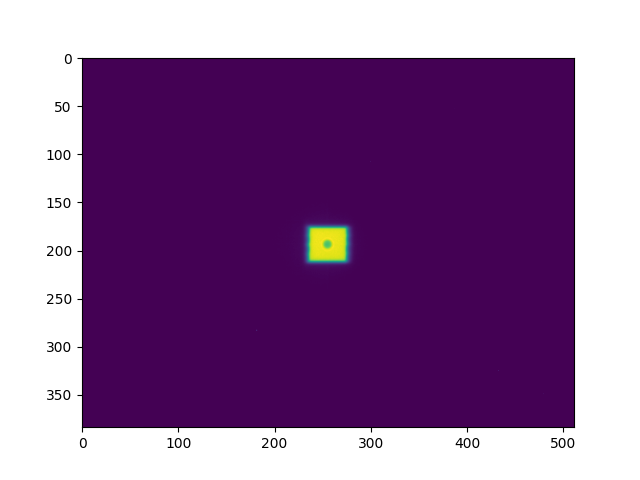
\includegraphics[width=\textwidth]{Content/Images/bb_find_algo_cropped_original.png}
            \caption{Original image}
        \end{subfigure}
        \begin{subfigure}[b]{0.49\textwidth}
            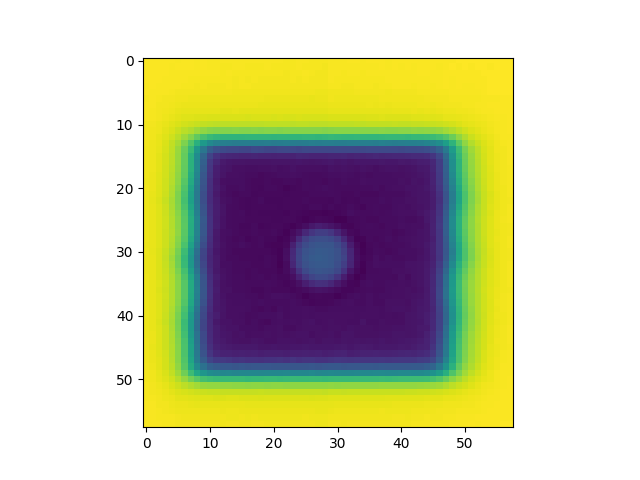
\includegraphics[width=\textwidth]{Content/Images/bb_find_algo_cropped_inverted.png}
            \caption{Cropped and inverted sample image}
        \end{subfigure}
        \caption{Cropping and invertion \cite{pylinac_images}}
    \end{figure}

    \item The sample is normalized to a range of 0-1. 

    \item The sample is converted to binary using thresholding. The threshold starts at a value of 0.02 and any pixel with a value below this is set to 0, otherwise, it is set to 1. Then each blob is checked if it passes all detection conditions. \emph{Detection conditions} are defined depending on the use case, and for the BB finding algorithm it is defined as

    \begin{enumerate}
        \item Blob is round,
        \item blob has an area within the expected range given by the BB size,
        \item blob has a circumference within the expected range given the BB size.
    \end{enumerate}

    \begin{figure}[H]
        \centering
        \begin{subfigure}[b]{0.40\textwidth}
            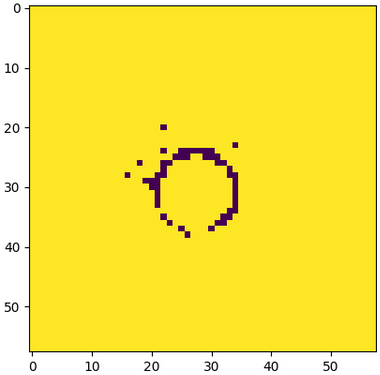
\includegraphics[width=\textwidth]{Content/Images/bb_find_algo_thresholding_low.png}
            \caption{Image at the start of the thresholding process}
        \end{subfigure}
        \begin{subfigure}[b]{0.40\textwidth}
            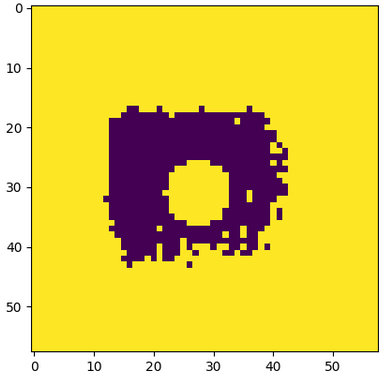
\includegraphics[width=\textwidth]{Content/Images/bb_find_algo_thresholding_high.png}
            \caption{Image after several thresholding process iterations}
        \end{subfigure}
        \caption{Thresholding \cite{pylinac_images}}
    \end{figure}
    
    If no blob passes all detection conditions, the threshold is increased by 0.02, and the detection process is repeated. If BB is detected, the thresholding algorithm will stop. If BB is not detected, the algorithm will continue until the threshold reaches 1.0.

    \item Center and boundary of detected BB is returned. If no BB is detected by then, error is raised.

    \begin{figure}[H]
        \centering
        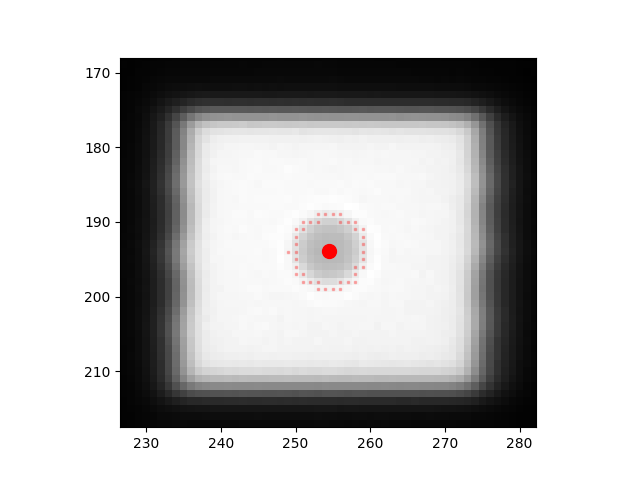
\includegraphics[width=0.7\textwidth]{Content/Images/bb_find_algo_thresholding_found.png}
        \caption{Image with found BB. \cite{pylinac_images}}
    \end{figure}
    
\end{enumerate}

\pagebreak

\subsection{Calculating couch shift} \label{subsec:couch_shift}

Geometric transformations of 2D planar images can be used to calculate shifts that could be applied to BB to match the radiation isocenter. \cite{low_et_al}. For each image $\mathbf{A}$ is needed to be determined:

\begin{equation}
    \mathbf{A}(\phi,\theta) = 
    \left(\begin{array}{ccc}
        -\cos(\phi) & -\sin(\phi) & 0\\
        -\cos(\theta)\sin(\phi) & \cos(\theta)\cos(\phi) & -\sin(\theta)\\
    \end{array} \right)
\end{equation}

where
\begin{itemize}
    \item $\theta$ is the gantry angle
    \item $\phi$ is the couch angle
\end{itemize}

Then, the $\xi$ matrix is calculated:

\begin{equation}
    \xi = (y_1, -x_1, ..., y_i, -x_i, ..., y_n, -x_n)^T
    \label{eq:cax_bb_shift_matrix}
\end{equation}

where $x_i$ and $y_i$ are the scalar shifts from the field CAX to the BB for $n$ images.

Having the above $\mathbf{B}(\phi_1, \theta_1, ...,\phi_n, \theta_n)$ can be calculated:

\begin{equation}
    \mathbf{B} = 
    \left(\begin{array}{c}
        \mathbf{A}(\phi_1, \theta_1) \\
        \vdots \\
        \mathbf{A}(\phi_i, \theta_i) \\
        \vdots \\
        \mathbf{A}(\phi_n, \theta_n) \\
    \end{array} \right)
\end{equation}

Shift vector $\mathbf{\Delta}$ can be solved using $\mathbf{B}$ and $\xi$:

\begin{equation}
    \mathbf{\Delta} = 
    \left(\begin{array}{c}
        \Delta Y \\
        \Delta X \\
        \Delta Z \\
    \end{array} \right)
\end{equation}

Couch shift calculation and algorithm descriptions based on \cite{pylinac_wl_algorithm}, which itself is based on \cite{winkler_et_al}, \cite{du_et_al} and \cite{low_et_al}.